\chapter{360度视频传输建模}
本论文把360度视频传输问题建模为一个多臂老虎机问题(MAB),并且使用了两层反馈来提高模型的效果。我们考虑单个用户通过无线信道从接入点下载全景视频。我们假设系统以时隙方式运行。在每个时隙,用户只能看到整个全景场景的一部分(通常为20\%),即视野(FoV)。如果用户的头部运动可以准确地预测,这样就足以提供20\%的全景图像,这大大降低了无线带宽消耗。不幸的是,很难准确预测用户的运动。因此,我们通常提供比FoV更大的部分来克服不准确的用户运动预测,但是增加传输的部分会使传输成功的可能性降低。因此我们需要正确的选择恰当的传输部分来最大化传输的吞吐量。


\section{视频传输的两层反馈}
在视频传输过程中,让$R(t)$表示将在时隙t中通过无线信道传输的全景图像部分的大小,因此我们称$R(t)$为$t$时隙的选择速度。我们假定$R(t)$只能从集合$\mathcal{R}=\left\{r_{1}, r_{2}, \ldots, r_{N}\right\}$中选择,其中$0<r_{1}<r_{2}<\cdots<r_{N}$。$r_{1}$和$r_{N}$分别表示FoV的大小和整个全景图片的大小。


第一个反馈是传输的全景视频块能否覆盖到用户的视野。我们使用$X_{n}(t)=1$标记$R(t) = r_{n}$足够的大以至于在时隙t被传输的块能够覆盖到用户的视野。反之$X_{n}(t)=0$则不能覆盖。让$\alpha_{n} \triangleq \operatorname{Pr}\left\{X_{n}(t)=1\right\}$做为预测成功率,显而易见$0<\alpha_{1}<\alpha_{2}<\cdots<\alpha_{N}$(因为传输的块越大,预测成功率越高)。在这里,由于用户的设备自动记录用户的当前位置(偏航、俯仰、滚动)并发送回AP(Access Point,接入点),因此AP在时隙t时,不管传输失败还是成功,都知道$X_{t}$的结果。


第二个反馈是传输是否成功。我们使用$C_{t}$来捕捉用户在时隙$t$时的信道衰落,假定其随时间独立且同相同的分布。我们并不能知道每一个时隙开始时的信道速率。如果所选择的传输速率并没有大于信道速率,即$R_{t} \leq C_{t}$,那无线传输在时隙t将会成功,否则失败。我们使用$Y_{n}(t) = 1$标记在时隙t通过选择速率$r_{t}$传输成功,$Y_{n}(t) = 1$则相反。让$\beta_{n} \triangleq \operatorname{Pr}\left\{Y_{n}(t)=1\right\}$表示传输成功概率。注意选择的速率越大,传输成功概率越低。因此,我们有$\beta_{1}>\beta_{2}>\cdots>\beta_{N}$。


\section{两层MAB模型}

在本文中,我们将交付部分选择问题描述为一个随机多臂老虎机(MAB)问题。MAB问题描述了一个玩家选择多个老虎机(Arm)的决策(Action)并从所选老虎机获得收益(Reward)的过程。在360度视频速率选择问题中,其中全景场景的不同交付部分,即不同的传输速率对应于不同的手臂(ARM)。Action是选择哪一个速率传输360度全景视频块。Reward对应传输系统的一段时间内累积吞吐量。我们的最终目标是在有限的时间范围内最小化遗憾(即,最佳累积吞吐量与算法下累积吞吐量之间的差距)。


J. Chen等人\cite{ref8}论述了两层反馈的MAB模型与传统的单反馈MAB模型的不同,并且证明了两层反馈的MAB模型的在360度视频传输问题中比单反馈MAB模型表现更优秀。我们的问题是两层反馈的MAB模型在容量发生周期性变化的信道上表现不是那么优秀。当信道容量发生改变时,两层反馈的MAB模型表现很迟钝,需要非常长的时隙才能输出正确的结果,即最佳传输速率。为此,我们基于两层反馈的MAB模型提出了多种改进算法,以便在信道容量发生改变时,能够更快适应信道并选择出更好的手臂,从而获得最小化遗憾。
\begin{figure}[h]
	\centering
	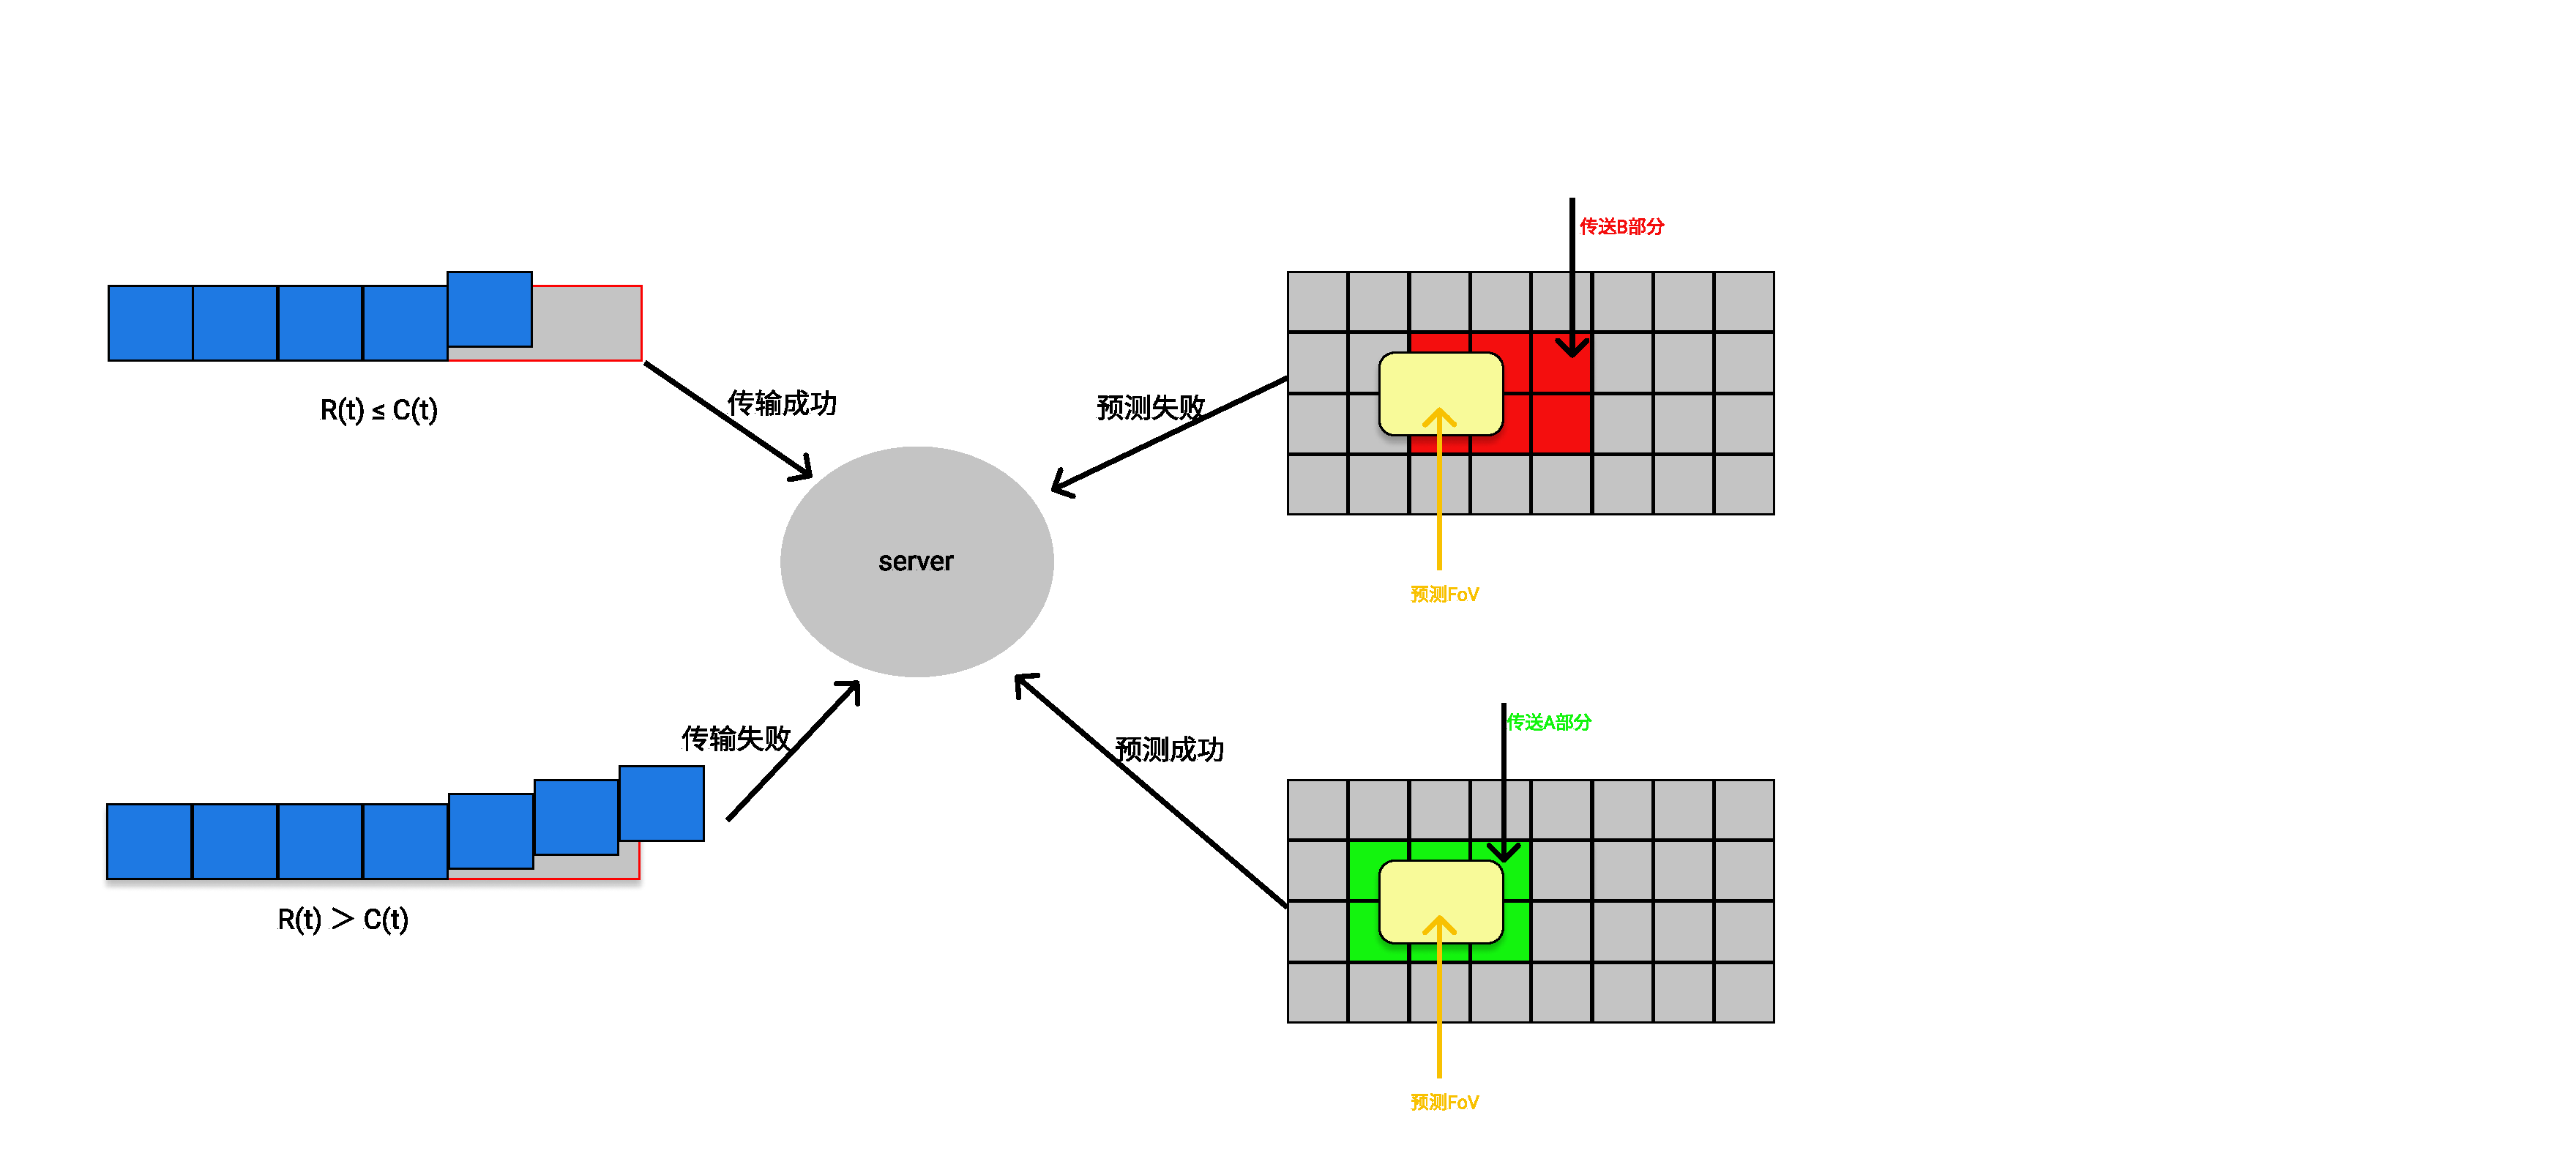
\includegraphics[width=0.8\textwidth]{figure/两层反馈.pdf}
	\caption{两层反馈示意图}
	\label{fig失败}
\end{figure}
在本文中,AP需要对选择的速率做出决定,以最大化系统吞吐量。如果用户的预测成功概率和传输成功概率(即$\left\{\alpha_{n}, \beta_{n}, n=1,2, \ldots, N\right\}$)都知道,则可通过解决以下优化问题来实现:
\begin{equation*}
n^{*} \in \underset{n=1,2, \ldots, N}{\arg \max } r_{n} \alpha_{n} \beta_{n},
\end{equation*}
其中$\alpha_{n} \triangleq \operatorname{Pr}\left\{X_{n}(t)=1\right\}$为预测成功率,$\beta_{n} \triangleq \operatorname{Pr}\left\{Y_{n}(t)=1\right\}$为传输成功概率,$r_{n}$表示全景图像传输部分的不同大小。然而预测和传输概率都是未知的,因为它们取决于许多因素,如用户行为、全景视频内容和无线环境。这要求算法不仅要学习这些统计数据,还要选择迄今为止的最佳速度。让$I(t) \in\{1,2, \ldots, N\}$表示t时刻所选择的速度的下标,我们的目的是设计一种学习算法,在一定的正整数时隙内实现最大的系统吞吐量。这相当于最小化遗憾,即累积吞吐量和最佳吞吐量之间的差距:
\begin{equation*}
\operatorname{Reg}(T) \triangleq \operatorname T{r}_{n^{*}} \alpha_{n^{*}} \beta_{n^{*}}-\mathbb{E}\left[\sum_{t=1}^{T} r_{I(t)} X_{I(t)}(t) Y_{I(t)}(t)\right].
\end{equation*}


如果在一个比较长的时间内遗憾过大,那就表明我们没有没有选择到最佳的传输速度。对用户而言,这往往意味着360度视频的传输延迟等,他/她的用户体验就大打折扣了。因此我们必须要达到一个次线性的遗憾才能够使得用户的体验最佳。
\section{本章小结}

本章对360度全景视频传输建模为两层反馈的MAB模型。在360度视频速率选择问题中,Arm对应不同的速率。Action是选择哪一个速率传输360度全景视频块。Reward对应传输系统的一段时间内累积吞吐量。我们也提出了两层反馈的MAB模型在周期信道上的局限性。我们的最终目标是开发一种算法,可以在时变带宽下快速确定一段时间内的最佳交付部分。下一章中详细描述如何基于两层反馈的MAB模型来改进获得表现更优秀的算法。

